\documentclass{seminar}

\usepackage[utf8]{inputenc}
\usepackage[T2A]{fontenc}
\usepackage[russian]{babel}
\usepackage{graphicx}
\usepackage{sem-a4}

\pagestyle{empty}

\begin{document}

\slideframe{none}
\sffamily

\begin{slide}

\center{Синтез и распознавание речи с открытыми исходными данными}
\center{Николай Шмырёв}
\center{nshmyrev@yandex.ru}
\center{http://voxforge.org}

\end{slide}

\begin{slide}

Речевые технологии

\begin{itemize}
\item Диалог с компьютером
\item Диктовка
\item Идентификация
\item Поддержка пользователей с ограниченными возможностями
\item Телекоммуникационные системы
\end{itemize}

\end{slide}

\begin{slide}

Синтез речи - Festival, MBROLA, Espeak

\end{slide}

\begin{slide}
Пакеты распознавания

\begin{itemize}
\item HTK
\item CMU Sphinx
\item ISIC
\item Julius
\end{itemize}

\end{slide}

\begin{slide}

Обучение программ и распознавание шаблонов (Pattern recognition)

\begin{itemize}
\item Шаблоны преобразования текста в произносимый текст
\item Шаблоны интонации
\item Шаблоны акустической информации
\item Шаблоны понимания (Common Sense)
\end{itemize}

\end{slide}

\begin{slide}

Проблема - базы данных для распознавания. Полноценные акустические базы существуют только
для английского языка. Есть русский, французский и испанский. 

Корень зла - http://www.ldc.upenn.edu/

Важны не только акустические, но и другие базы - фонетические словари, 
интонационно размеченные записи, смысловые базы.

Создание базы - очень дорогостоящий и трудоёмкий процесс. Например, разметка
минуты речи специалистом занимает около получаса.

\end{slide}

\begin{slide}
http://www.espgame.org/

Luis Von Ahn. Human Computation (Google Tech Talks)

\begin{figure}
\begin{center}
\includegraphics[width=.9\textwidth]{./images/esp.eps}
\end{center}
\end{figure}

\end{slide}

\begin{slide}

http://freesound.iua.upf.edu

\begin{figure}
\begin{center}
\includegraphics[width=.9\textwidth]{./images/freesound.eps}
\end{center}
\end{figure}

\end{slide}

\begin{slide}

http://voxforge.org

\begin{figure}
\begin{center}
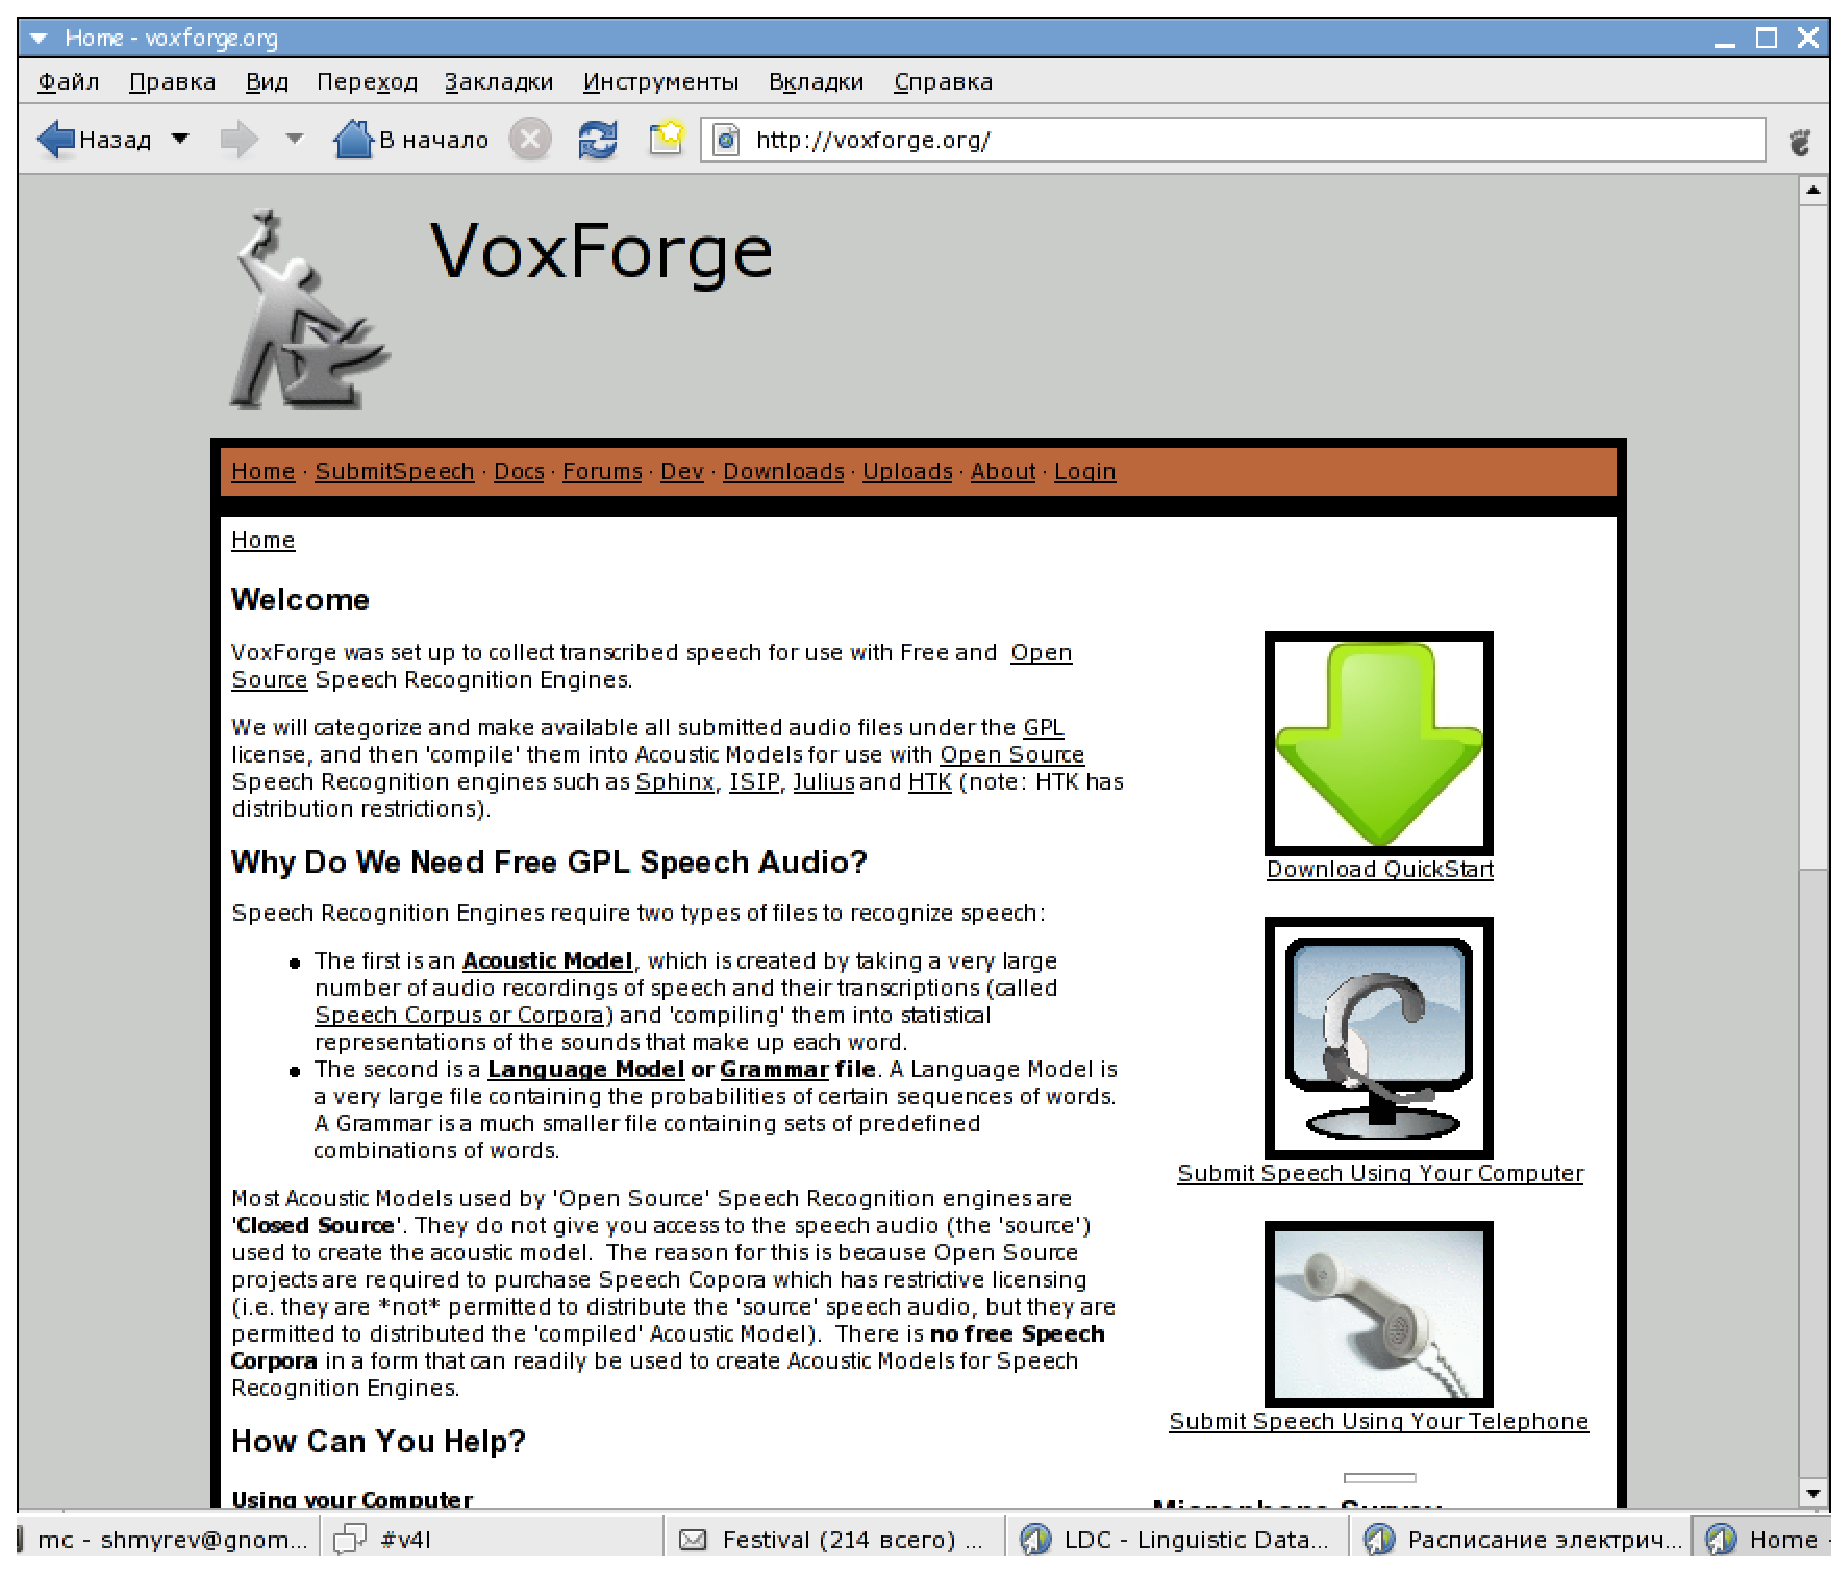
\includegraphics[width=.7\textwidth]{./images/voxforge.eps}
\end{center}
\end{figure}

\end{slide}


\begin{slide}
gnome-voice-control. Google SOC

\begin{itemize}
\item Управление рабочим столом
\item Управление приложениями
\item Диктовка
\item Поддержка нескольких языков
\end{itemize}

\end{slide}

\end{document}
